\PassOptionsToPackage{svgnames,dvipsnames}{xcolor}
\documentclass[aspectratio=169]{beamer}
\usepackage{microtype}

\usetheme{moloch}
\setbeamertemplate{page number in head/foot}[appendixframenumber]
\setbeamertemplate{frame footer}{%
    \insertsectionnumber{}. \insertsectionhead{}%
    \ifx\insertsubsectionhead\empty\relax\else$\ \vartriangleright{}\ $\insertsubsectionhead\fi
}

\usepackage{biblatex}
\addbibresource{main.bib}

\title{Mechanized semantics for ECMAScript regexes}
\subtitle{Master Project Defense}
\author{No\'{e} De Santo}
\institute{EPFL}
\date{February 15, 2024}

\newcommand\todo[1]{\textcolor{red}{#1}}

\usepackage{booktabs}
\usepackage{listings}
\usepackage{lstcoq}
\def\inlinecode#1{\lstinline[language=Coq,basicstyle=\ttfamily]{#1}}


\lstset{
    basicstyle=\ttfamily,
    keepspaces=true,
    columns=fixed,
    lineskip=-0.5pt,
    %breaklines=true
}
\lstdefinelanguage{ocaml} {
    basicstyle=\ttfamily,
    morekeywords={let},
    identifierstyle={\ttfamily\color{black}},
    keywordstyle={\ttfamily\color{Maroon}},
    stringstyle=\color{OliveGreen},
    showstringspaces=false,
    morestring=[d]",
    morestring=[d]',
    morestring=[s]{\{|}{|\}},
}

% \addtobeamertemplate{block example begin}{\pgfsetfillopacity{0.5}}{\pgfsetfillopacity{1}}
\setbeamercolor{block title example}{bg=example text.fg!40}
\setbeamercolor{block body example}{bg=example text.fg!10}

\usepackage{cleveref}


% Regex constructs
\usepackage{xifthen}

\newcommand{\eps}[0]{\varepsilon}
\newcommand{\hole}[0]{\square}
\newcommand{\charclass}[1]{[#1]}
\newcommand{\ncharclass}[1]{\charclass{\widehat{\phantom{x}}#1}}
\newcommand{\dotc}[0]{{\cdot{}}}
\newcommand{\escaped}[1]{\backslash{}#1}
\newcommand{\disj}[0]{\mathbin{|}}
\renewcommand{\star}[0]{^{*}}
\newcommand{\plus}[0]{^{+}}
\newcommand{\lazystar}[0]{^{*?}}
\newcommand{\lazyplus}[0]{^{+?}}
\newcommand{\question}[0]{^{?}}
\newcommand{\frep}[1]{^{\{#1\}}}
\newcommand{\rrep}[2]{^{\{#1,#2\}}}
\newcommand{\lstar}[0]{^{*?}}
\newcommand{\lplus}[0]{^{+?}}
\newcommand{\lquestion}[0]{^{??}}
\newcommand{\lfrep}[1]{^{\{#1\}?}}
\newcommand{\lrrep}[2]{^{\{#1,#2\}?}}
\newcommand{\pgroup}[1]{({?}{:}\ #1)}
\newcommand{\group}[2][]{(\ifthenelse{\equal{#1}{}}{}{_{\textup{\scriptsize<#1>}}}#2)}
\newcommand{\mstart}[0]{\widehat{\phantom{x}}}
\newcommand{\mend}[0]{\mathdollar}
\newcommand{\wboundary}[0]{\escaped{\textup{b}}}
\newcommand{\wBoundary}[0]{\escaped{\textup{B}}}
\newcommand{\lookahead}[1]{({?}{=}\ #1)}
\newcommand{\lookbehind}[1]{({?}{\leq}\ #1)}
\newcommand{\neglookahead}[1]{({?}{\not=}\ #1)}
\newcommand{\neglookbehind}[1]{({?}{\not\leq}\ #1)}
\newcommand{\nbackref}[1]{\escaped{\textup{<#1>}}}
\newcommand{\backref}[1]{\escaped{\textup{#1}}}

\newcommand{\agroup}[1]{({?}{>}\ #1)}
\newcommand{\balgroup}[3]{\group[#1-#2]{#3}}
\newcommand{\recursion}[1]{({?}#1)} % Also called subroutine
\newcommand{\callout}[1]{({?}C_{\textup{#1}})}

\usepackage{tikz}
\usepackage{pgfplots} 
\usetikzlibrary{positioning,decorations.pathreplacing,calc}
\usetikzlibrary{overlay-beamer-styles}
\usepackage{forest}
\usepackage{prftree}

\newcommand{\okcheck}[0]{\textcolor{\codehgcolorG}{\checkmark{}}}
\newcommand{\nocheck}[0]{\textcolor{\codehgcolorR}{\raisebox{\depth}{$\chi{}$}}}

\newcommand{\rulesep}[0]{\quad{}||\quad{}}

\newcommand{\overgroup}[4][]{\draw [decorate,decoration={brace,amplitude=1},thick,#1] (char#2.north west) --node[above]{#4} (char#3.north east);}
\newcommand{\undergroup}[4][]{\draw [decorate,decoration={brace,amplitude=1,mirror},thick,#1] (char#2.south west) --node[below]{#4} (char#3.south east);}
\newenvironment{match}[2]{%
\begin{tikzpicture}[baseline=0pt]%
    \foreach \n [count=\i from 0] in {``,#1,''} {%
        \node [anchor=base, text height=2ex, text depth=0.5ex, inner sep=1.5pt] (char\i) at (\i*1 em,0) {\n};  %
    }%
    \draw [very thick] ([yshift=0.5ex]char1.south west) -| (char#2.east);%
}{\end{tikzpicture}}
\newcommand{\simplematch}[2]{\begin{match}{#1}{#2}\end{match}}

\begin{document}
    \maketitle

    \section{Introduction}

    \begin{frame}{Regular expressions}
        \makebox[\textwidth][s]{Regular expressions as originally defined by Kleene~\cite{kleene} and used in automata theory~\cite{Edelmann,intro_automata}.}
        \pause{}%
        \begin{align*}
            a \in  \Sigma \qquad{} r \mathrel{::=}  a \rulesep{} \eps{} \rulesep{} r_1 r_2 \rulesep{} r_1 \disj{} r_2 \rulesep{} r\star{}
        \end{align*}
        \pause{}%
        \begin{gather*}
            \prfaxiom{a \vdash{} \text{``a''}} \qquad{}
            \prfaxiom{\eps{} \vdash{} \text{``''}} \qquad{}
            \prftree{\prfassumption{r_1 \vdash{} v}}{\prfassumption{r_2 \vdash{} w}}{r_1r_2 \vdash{} vw} \\
            \prftree{\prfassumption{r_1 \vdash{} v}}{r_1 \disj{} r_2 \vdash{} v} \qquad{}
            \prftree{\prfassumption{r_2 \vdash{} v}}{r_1 \disj{} r_2 \vdash{} v} \\
            \prfaxiom{r\star{} \vdash{} \text{``''}} \qquad{}
            \prftree{\prfassumption{r \vdash{} v}}{\prfassumption{r\star{} \vdash{} w}}{r\star{} \vdash{} vw}
        \end{gather*}
        % \begin{minipage}{0.40\textwidth}
        %     \pause{}
        %     \begin{align*}
        %         \mathcal{L}(a) \mathrel{:=}& \{ \text{``a''} \} \\
        %         \mathcal{L}(\eps{}) \mathrel{:=}& \{ \text{``''} \} \\
        %         \mathcal{L}(r_1 r_2) \mathrel{:=}& \{vw \mid{} v \in{} \mathcal{L}(r_1) \land{} w \in \mathcal{L}(r_2) \} \\
        %         \mathcal{L}(r_1 \disj{} r_2) \mathrel{:=}& \mathcal{L}(r_1) \cup{} \mathcal{L}(r_2) \\
        %         \mathcal{L}(r\star{}) \mathrel{:=}& \bigcup\nolimits_{i = 0}^\infty{} r^i&
        %     \end{align*}
        % \end{minipage}
    \end{frame}

    \begin{frame}{Regexes are not Regular Expressions (anymore)}
        Regexes as in PCRE2,Perl,JavaScript,Java,.NET,Python,Rust,\ldots{}
        \pause{}
        \begin{align*}
            r \mathrel{::=}
            && & a \\
            &&\rulesep{}& [a_1-a_2] \\
            &&\rulesep{}& \escaped{b} \rulesep{} \ldots \\
            &&\rulesep{}& r_1 r_2 \\
            &&\rulesep{}& r_1 \disj{} r_2 \\
            &&\rulesep{}& r\star \rulesep{} r\plus{} \rulesep{} r\question{} \rulesep{} r\rrep{\mathbb{N}}{\mathbb{N}} \\
            &&\rulesep{}& r\star \rulesep{} r\lplus{} \rulesep{} r\lquestion{} \rulesep{} r\lrrep{\mathbb{N}}{\mathbb{N}} \\
            &&\rulesep{}& \group{r} \rulesep{} \group[name]{r} \rulesep{} \\
            &&\rulesep{}& \escaped{\mathbb{N}} \rulesep{} \nbackref{name} \\
            &&\rulesep{}& \lookahead{r} \rulesep{} \neglookahead{r} \rulesep{} \lookbehind{r} \rulesep{} \neglookbehind{r} % \\
            % &&\rulesep{}& \mstart{} \rulesep{} \mend{} \rulesep{} \wboundary{} \rulesep{} \wBoundary \\
            % &&\rulesep{}& \agroup{r} \\
            % &&\rulesep{}& \balgroup{name1}{name2}{r} \\
            % &&\rulesep{}& \recursion{\mathbb{N}} \rulesep{} \recursion{{+}\mathbb{N}} \rulesep{} \recursion{{-}\mathbb{N}} \rulesep{} \\
            % &&\rulesep{}& \callout{name} \\
            % &&\rulesep{}& \ldots{}
        \end{align*}
    \end{frame}
    \begin{frame}{Regexes are not Regular Expressions (anymore)}
        \begin{align*}
            \phantom{r \mathrel{::=}} && & \phantom{\lookahead{r} \rulesep{} \neglookahead{r} \rulesep{} \lookbehind{r} \rulesep{} \neglookbehind{r}} \\
            &&\rulesep{}& \mstart{} \rulesep{} \mend{} \rulesep{} \wboundary{} \rulesep{} \wBoundary \\
            &&\rulesep{}& \agroup{r} \\
            &&\rulesep{}& \balgroup{name1}{name2}{r} \\
            &&\rulesep{}& \recursion{\mathbb{N}} \rulesep{} \recursion{{+}\mathbb{N}} \rulesep{} \recursion{{-}\mathbb{N}} \rulesep{} \\
            &&\rulesep{}& \callout{name} \\
            &&\rulesep{}& \ldots{}
        \end{align*}
    \end{frame}

    \begin{frame}{Differences between regex languages}
        What about semantics?
        \pause{}
        \begin{itemize}
            \item $a \disj{} ab$ on ``ab''.
            \pause{}
            \begin{itemize}
                \item Posix (ERE): \simplematch{a,b}{2}
                \item JavaScript: \simplematch{a,b}{1}
            \end{itemize}
            \vspace{3em}\pause{}
            \item $\pgroup{\group{a} \disj{} b}\star{}$ on ``ab''.
            \pause{}
            \begin{itemize}
                \item Python,Rust,.Net,\ldots:
                    \begin{match}{a,b}{2}
                        \overgroup{1}{1}{1}
                    \end{match}
                \item JavaScript: \simplematch{a,b}{2} (nothing was captured)
            \end{itemize}
        \end{itemize}
    \end{frame}

    \begin{frame}{A specification of Regexes}
        \begin{itemize}
            \item JavaScript has a specification: ECMAScript.
            \pause{}
            \item ECMAScript specifies the semantics of its regexes.
        \end{itemize}
    \end{frame}

    \begin{frame}{Goals \& benefits}
        \emph{Goal:} mechanize the section about regexes of the ECMAScript specification in the Coq proof assistant.

        \pause{}
        \emph{Mechanization benefits:}
        \begin{itemize}
            \item Foundation for formal reasoning about JavaScript regexes;
            \pause{}
            \item Provide a better understanding of implicit invariants of the specification;
            \pause{}
            \item An executable ``ground truth''.
        \end{itemize}
    \end{frame}

    \begin{frame}{State of the art}
        \begin{itemize}
            \item The ECMAScript specification has already been mechanized many times~\cite{jscert,lambdajs,aplas_js,kjs}\ldots{}
            \pause{}
            but the section on regexes was not.
            \pause{}
            \item Alternative equivalent semantics for regexes are sometimes defined in the literature~\cite{expose,repair_dos}\ldots{}
            \pause{}
            but these typically get details wrong, e.g.
            \[e\question{} \equiv{} e \disj{} \eps{} \]
            does not hold.
        \end{itemize}
    \end{frame}

    \begin{frame}{Results}
        A reasonably future-proof, proven-safe, executable mechanization of the ECMAScript regexes.
        \pause{}
        \begin{itemize}
            \item Mechanizing the ECMAScript regex specification in the Coq proof assistant (\cref{sec:mechanization});
            \pause{}
            \item Using this mechanized specification: proofs (\cref{sec:proofs}) that
                \begin{itemize}
                    \item Matching always terminate;
                    \item No operation ever fails, e.g.
                        \begin{itemize}
                            \item Assertions;
                            \item List indexing.
                        \end{itemize}
                \end{itemize}
            \pause{}
            \item Extracting an executable engine in OCaml (\cref{sec:conclusion}).
        \end{itemize}
    \end{frame}

    \section{ECMA Regexes}

    \begin{frame}{Features: overview}
        \begin{center}
            \begin{tabular}{lcc}
                Feature name & Syntax \\ \toprule
                Character & a, b, c, $\escaped{n}$, \ldots \\
                Character classes & $\charclass{abc}$, $\ncharclass{A-Z}$, $\dotc{}$, $\escaped{d}$, \ldots \\
                Sequence/concatenation & $r_1 r_2$ \\
                Disjunction/union & $r_1 \disj{} r_2$ \\
                Greedy quantifiers & $r\star{}$, $r\plus{}$, $r\question{}$, $r\rrep{\mathbb{N}}{\mathbb{N}}$, \ldots \\
                Lazy quantifiers & $r\lstar{}$, $r\lplus{}$, $r\lquestion{}$, $r\lrrep{\mathbb{N}}{\mathbb{N}}$, \ldots \\
                Capturing groups & $\group{r}$, $\group[name]{r}$ \\
                Non-capturing groups & $\pgroup{r}$ \\
                Backreferences & $\escaped{\mathbb{N}}$, $\nbackref{name}$ \\
                Lookarounds & $\lookahead{r}$, $\lookbehind{r}$, $\neglookahead{r}$, $\neglookbehind{r}$ \\
                Anchors & $\mstart{}$, $\mend{}$, $\wboundary{}$, $\wBoundary{}$
            \end{tabular}\\[0.4em]
        \end{center}
    \end{frame}

    \begin{frame}{Features: close-up view}
        \begin{itemize}
            \item<1->
                \textbf{Quantifiers:} Allow to repeat another regex repeatedly, e.g. $\star{}$, $\plus{}$, and $\question{}$.
                ECMAScript also offers \emph{bounded} quantifiers.
                \only<1>{
                    \\E.g. $a\rrep{4}{}$ matches `a' as many times as possible, and at least 4 times.\\
                    \begin{center}
                    \begin{tabular}{ll}
                        ``aa'' & \nocheck{} \\
                        ``aaaa'' & \okcheck{} \\
                        ``aaaaaaaaaaa'' & \okcheck{}
                    \end{tabular}
                    \end{center}}
                    
            \item<2->
                \textbf{Capturing groups:} Allow to retrieve strings matched by sub-parts of the regex.
                \only<2>{
                    \\E.g. $\textcolor{red}{(}\textcolor{blue}{(}a\star{}\textcolor{blue}{)}\textcolor{green}{(}b\star{}\textcolor{green}{)}\textcolor{red}{)}$ on ``aaba'' \pause{}yields
                    \begin{match}{a,a,b,a}{3}
                        \undergroup[draw=red,text=red]{1}{3}{1}
                        \overgroup[draw=blue,text=blue]{1}{2}{2}
                        \overgroup[draw=green,text=green]{3}{3}{3}
                    \end{match}
                    \pause{}
                    \\Groups are numbered in order of appearance of their left parenthesis.}
            \item<3->
                \textbf{Non-capturing groups:} Allow to override the operators' precedence.
                \\E.g. $\pgroup{a \disj{} b} c \quad{}\not\equiv{}\quad{} a \disj{} bc \quad{}\equiv{}\quad{} a \disj{} \pgroup{bc}$
        \end{itemize}    
    \end{frame}

    \begin{frame}{Pipeline}
        \begin{itemize}
            \item ECMAScript regexes: \textasciitilde{}50 pages; pseudo-code for a backtracking-based matching algorithm.
            \pause{}
            \item Describes the following pipeline:\\[1em]
            \begin{tikzpicture}[node distance=20pt]
                \node [draw, fill=gray, fill on=<4->] (parse) {Parsing};
                \node [draw, right=of parse, fill=\codehgcolorG, fill opacity=0.8, text opacity=1.0, fill on=<4->] (ee) {Early Errors};
                \node [draw, right=of ee, fill=\codehgcolorG, fill opacity=0.8, text opacity=1.0, fill on=<4->] (compile) {Compilation};
                \node [draw, right=of compile, fill=\codehgcolorG, fill opacity=0.8, text opacity=1.0, fill on=<4->] (exec) {Matching};

                \node [below left=of parse] (regex_lit) {$a \disj{} b$};
                \node [below=of exec] (input) {(``ab'',0)};
                \node [below right=of exec] (output) {} [sibling distance = 0.75em, level distance = 5pt,edge from parent/.style={}]
                    child { node[anchor=base, text height=2ex, text depth=0.5ex, inner sep=1.5pt] {``} } % ''
                    child { node[anchor=base, text height=2ex, text depth=0.5ex, inner sep=1.5pt] (match) {a} }
                    child { node[anchor=base, text height=2ex, text depth=0.5ex, inner sep=1.5pt] {b} }
                    child { node[anchor=base, text height=2ex, text depth=0.5ex, inner sep=1.5pt] {''} };
                
                \draw [-stealth] (parse) -- (ee)
                    node [midway, below=10pt] {$\hole{} \disj{} \hole{}$} [sibling distance = 25pt, level distance = 25pt, edge from parent/.style={draw,-}]
                        child { node [text height=2ex] {$a$} }
                        child { node [text height=2ex] {$b$} };
                \draw [-stealth] (ee) -- (compile)
                    node [midway, below=10pt] {\okcheck{}};
                \draw [-stealth] (compile) -- (exec)
                    node [midway, below=10pt] {m};
                \draw [-stealth] (input) -- (exec);

                \draw [-stealth] (regex_lit) |- (parse);
                \draw [-stealth] (exec) -| (output);

                \draw [very thick] ([yshift=0.5ex]match.south west) -| (match.east);
            \end{tikzpicture}
        \end{itemize}
        \only<3>{%
            Early errors: $a\rrep{3}{2}$, $\group{a}\backref{2}$}
        \only<4>{%
            The mechanization does not include Parsing.\\
            In this presentation, we will focus on compilation and matching.}
    \end{frame}

    \begin{frame}{Compilation\&matching: state}
        The specification needs types to represent the (internal) state of the match.
        \lstinputlisting[language=Coq]{listings/compilation_and_matching/types_state.v}
        \only<2-3>{%
            E.g.\ \inlinecode{MatchState}:\\
            \begin{match}{a,a,b,b,b,a,c}{3}
                \overgroup{2}{3}{1}
            \end{match}
            \only<3>{\\
                is represented as\\
                (``aabbbac'', 3, $\{\#_1 \mapsto{} [1,2], \#_2 \mapsto{} \texttt{undefined}$\})}}
        \only<4>{%
            E.g.\ \inlinecode{MatchResult}:\\
            \texttt{Some} (``aabbbac'', 3, $\{\#_1 \mapsto{} [1,2], \#_2 \mapsto{} \texttt{undefined}$\})\\
            or\\
            \texttt{mismatch} (a.k.a. \texttt{None})}
    \end{frame}

    \begin{frame}{The compilation phase}
        The main compilation function: \inlinecode{compileSubpattern: Regex -> Matcher}.

        Defined recursively on the regex being compiled.
    \end{frame}

    \begin{frame}{Compilation\&matching: example}
        Consider $\pgroup{a \disj{} b}c$. It could be compiled as follows:
        \only<2-4>{\lstinputlisting[language=Coq]{listings/compilation_and_matching/matcher.v}}
        \only<5->{\lstinputlisting[language=Coq]{listings/compilation_and_matching/matcher_hg.v}}
        \vspace{-1em}
        \only<3->{\lstinputlisting[language=Coq]{listings/compilation_and_matching/continuation.v}}
        \only<4->{A match would be found by calling, e.g. \inlinecode{m ("abc", 1, NoCaptures) k}.}
    \end{frame}

    \section{Mechanization}\label{sec:mechanization}

    \begin{frame}{Literate mechanization}
        \only<1-2>{%
            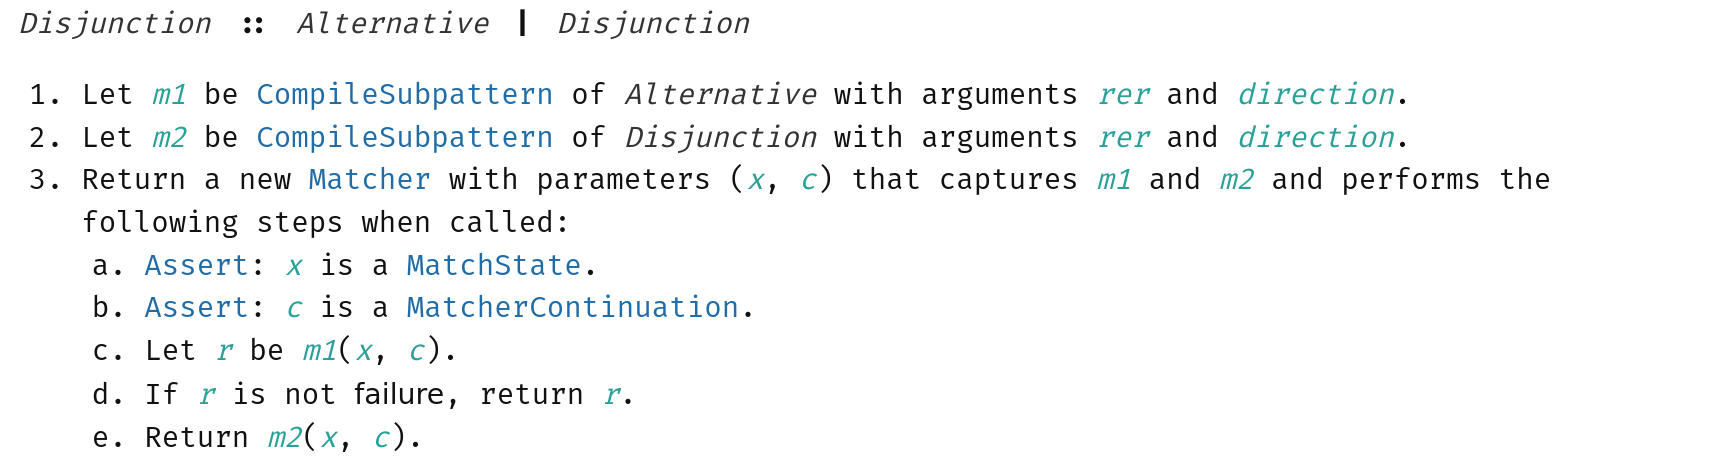
\includegraphics[width=\textwidth]{pics/ecma_spec/disjunction.png}}
        \only<2>{%
            \lstinputlisting[language=Coq,basicstyle=\ttfamily\scriptsize]{listings/mechanization/disjunction.v}}
        \only<3->{%
            \lstinputlisting[language=Coq,basicstyle=\ttfamily\scriptsize,breaklines]{listings/mechanization/disjunction_literate.v}
        \only<4>{But of course not everything can be directly translated.}}
    \end{frame}

    \begin{frame}{Problem 1: the specification uses fallible operations}
        \begin{center}
            \only<1>{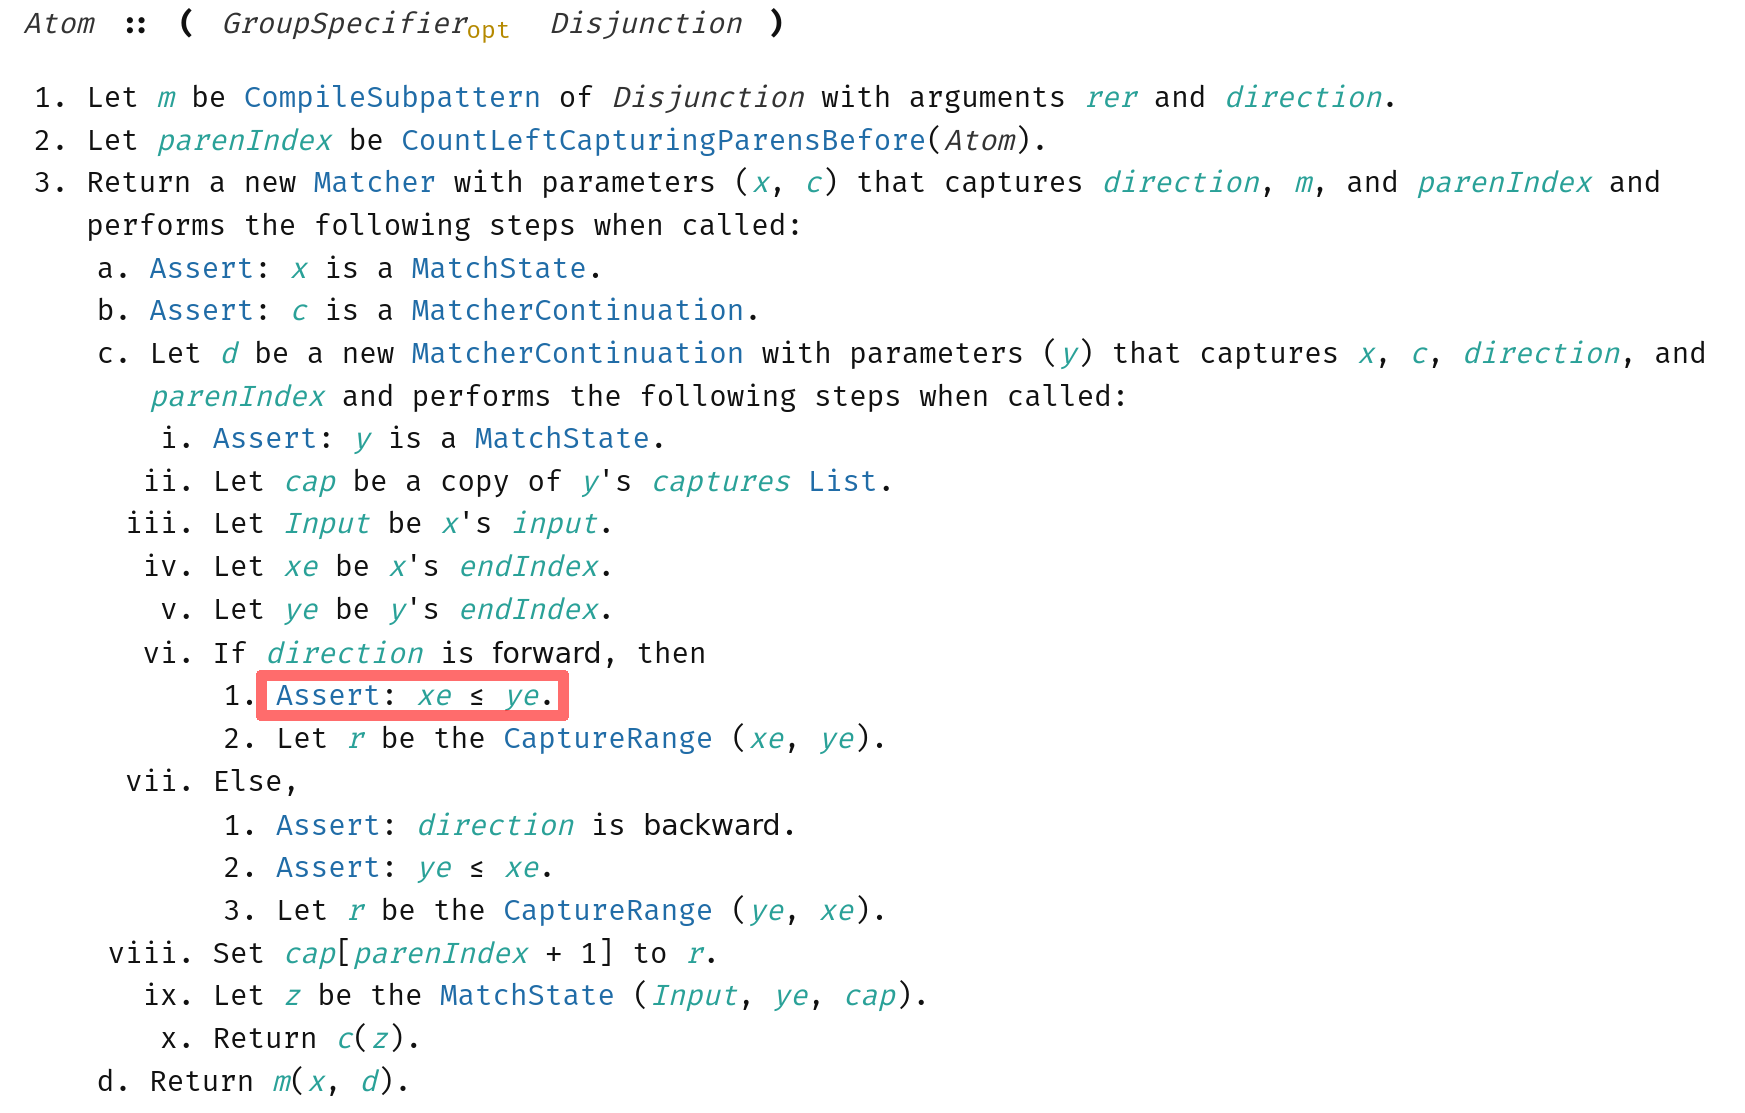
\includegraphics[width=0.8\textwidth]{pics/ecma_spec/groups_hg_1.png}}
            \only<2>{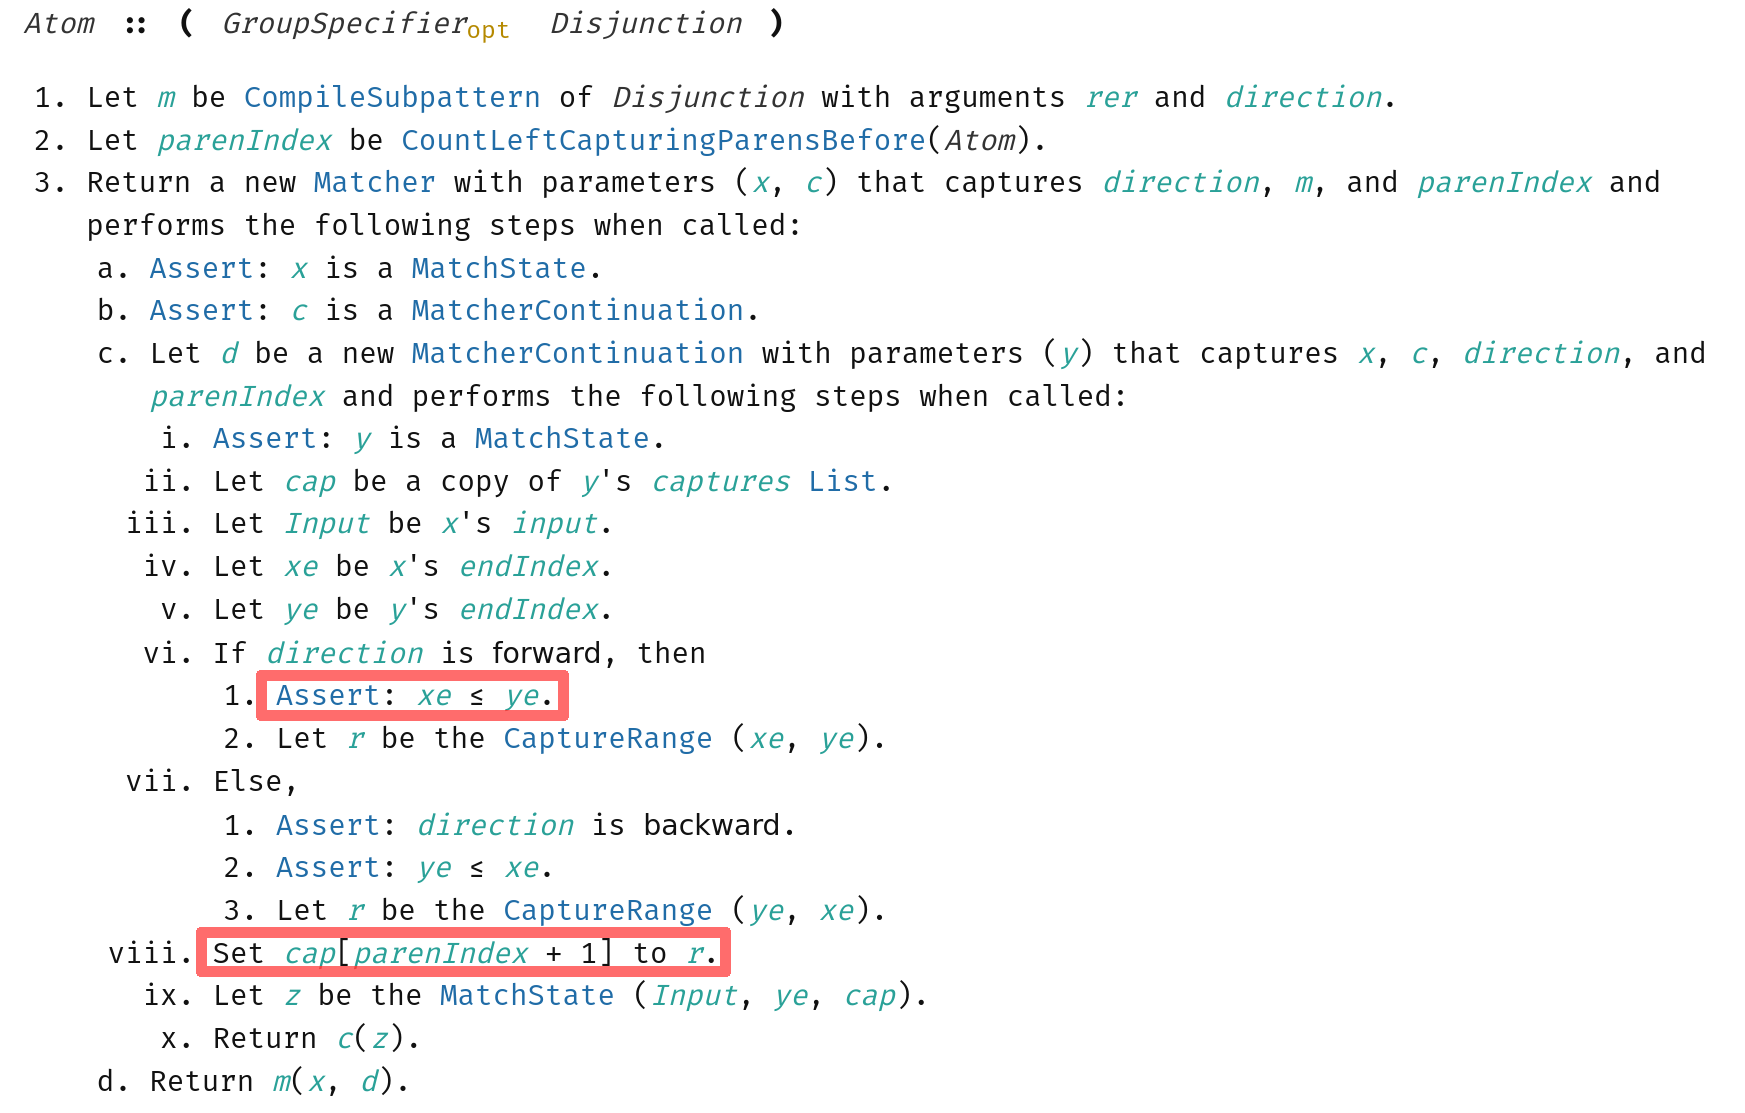
\includegraphics[width=0.8\textwidth]{pics/ecma_spec/groups_hg_2.png}}
        \end{center}
    \end{frame}

    \begin{frame}{Solution 1: encoding failures --- the error monad}
        Wrap the result of computations which can fail in the error monad~\cite{monads_wadler}.
        \lstinputlisting[language=Coq]{listings/error_monad/definition.v}
    \end{frame}

    \begin{frame}{Solution 1: encoding failures --- mechanizing}
        \lstinputlisting[language=Coq]{listings/solutions/errors.v}
    \end{frame}

    \begin{frame}{Solution 1: encoding failures --- notations}
        \lstinputlisting[language=Coq]{listings/error_monad/notations.v}
    \end{frame}

    \begin{frame}{Solution 1: encoding failures --- end result}
        \lstinputlisting[language=Coq]{listings/solutions/notations.v}
    \end{frame}

    \begin{frame}{Problem 2: unbounded recursion}
        General recursion is needed to implement quantifiers, e.g. $e\rrep{\texttt{min}}{}$\\
        \qquad{}$\implies{}$ not structurally recursive.
        \pause{}

        \lstinputlisting[language=Coq,basicstyle=\ttfamily\small]{listings/repeat_matcher/definition_nofuel.v}
    \end{frame}

    \begin{frame}{Solution 2: encoding (non-)termination --- fuel}
        \lstinputlisting[language=Coq,basicstyle=\ttfamily\small]{listings/repeat_matcher/definition.v}
        \pause{}
        \begin{center}\begin{tabular}{c}
            The (original) function terminates\\
            $\iff{}$\\
            \lstinline[language=Coq,basicstyle=\small]{\\exists fuel, RepeatMatcher m min x c fuel <> Failure OutOfFuel}.
        \end{tabular}\end{center}
    \end{frame}

    \begin{frame}{Problem 3: missing arguments}
        \begin{minipage}{0.4\textwidth}
            \begin{forest}
                [$\square \square$, name=root
                [$\square | \square$
                    [$(\square)$, name=g1 [$a$]]
                    [$(\square)$, name=g2 [$a$]]]
                [$b$]
                ]
                \node[left = 0.5cm of root] (root_label) {$r$ (root)};
                \draw[->] (root_label) to[out = east, in = west] (root);
                \node[left = 0.25cm of g1] (g1_label) {$r_1$};
                \draw[->] (g1_label) to[out = east, in = west] (g1);
                \node[right = 0.25cm of g2] (g2_label) {$r_2$};
                \draw[->] (g2_label) to[out = west, in = east] (g2);
            \end{forest}
        \end{minipage}
        \begin{minipage}{0.57\textwidth}
            How to compute the group index of \inlinecode{r2}?
            \pause{}
            
            \inlinecode{countLeftParenthesesBefore r2 = 1}
        \end{minipage}
    \end{frame}

    \begin{frame}{Solution 3: encoding the context --- zipper}
        Use a zipper~\cite{zipper} to represent a regex and its context.
        \inlinecode{RegexNode := (Regex * list RegexContext)}
        \vfill{}

        \only<1>{%
            \hfill{}
            \begin{minipage}{0.3\linewidth}
            \begin{forest}
                for tree={text=orange, edge=gray},
                [$\square b$, name=root
                [$\square | (a) $
                    [$(\square)$, name=g1,for tree={text=black}, for descendants={edge=black}, [$a$]]]]
                \node[left = 0.5cm of g2] (g1_label) {$r_1$};
                \draw[->] (g1_label) to[out = east, in = west] (g1);
            \end{forest}
            \end{minipage}
            \hfill
            \begin{minipage}{0.3\linewidth}
            \begin{forest}
                for tree={text=orange, edge=gray},
                [$\square b$, name=root
                [$(a) | \square$
                    [$(\square)$, name=g2,for tree={text=black}, for descendants={edge=black}, [$a$]]]]
                \node[right = 0.5cm of g2] (g2_label) {$r_2$};
                \draw[->] (g2_label) to[out = west, in = east] (g2);
            \end{forest}
            \end{minipage}
            \hfill{}}
        \only<2>{%
            \lstinputlisting[language=Coq]{listings/solutions/context.v}}
        \vfill{}
    \end{frame}

    \section{Proofs}\label{sec:proofs}

    \begin{frame}{Goals}
        We want to prove two things:
        \begin{itemize}
            \item The matching process always terminate;
            \item No operation ever fails during matching.
        \end{itemize}
    \end{frame}

    \begin{frame}{Mechanized invariant}
        The matcher invariant will be instrumental to proving both termination and the absence of failures.

        \lstinputlisting[language=Coq]{listings/matcher_invariant.v}
        where \inlinecode{x <= y} $\iff$ \inlinecode{EndIndex x <= EndIndex y}.
    \end{frame}

    \begin{frame}{Proving the invariant}
        \lstinputlisting[language=Coq]{listings/matcher_invariant/compilation.v}
        By induction on \inlinecode{r}.
    \end{frame}

    \begin{frame}{Proving the invariant: RepeatMatcher}
        %Assuming \inlinecode{m} satisfies the matcher invariant,
        %does \inlinecode{RepeatMatcher m min x c fuel} result either in a \inlinecode{mismatch} or a call to \inlinecode{c}?
        \only<1>{\lstinputlisting[language=Coq,basicstyle=\ttfamily\small]{listings/repeat_matcher/analysis/step_1.v}}
        \only<2>{\lstinputlisting[language=Coq,basicstyle=\ttfamily\small]{listings/repeat_matcher/analysis/step_2.v}}
        \only<3>{\lstinputlisting[language=Coq,basicstyle=\ttfamily\small]{listings/repeat_matcher/analysis/step_3.v}}
        \only<4>{\lstinputlisting[language=Coq,basicstyle=\ttfamily\small]{listings/repeat_matcher/analysis/step_4.v}}
        \only<5>{\lstinputlisting[language=Coq,basicstyle=\ttfamily\small]{listings/repeat_matcher/analysis/step_5.v}}
        \only<6->{\lstinputlisting[language=Coq,basicstyle=\ttfamily\small]{listings/repeat_matcher/analysis/step_6.v}}

        \only<6>{\centering If \inlinecode{min + remainingChars(x) + 1 <= fuel}.}
    \end{frame}

    \begin{frame}{Proving termination (for free)}
        \lstinputlisting[language=Coq]{listings/termination/statement.v}
        \pause{}
        Direct if \inlinecode{m x (fun z => Success z) = mismatch <> Failure _}.
        Otherwise, by the matcher invariant, for some \inlinecode{y}\\
        \begin{tabular}{ll}
            \lstinline[language=Coq]{m x (fun z => Success z)} & \inlinecode{= (fun z => Success z) y} \\
            & \inlinecode{= Success y} \\
            & \inlinecode{<> Failure _}
        \end{tabular}\\
        \qed{}
    \end{frame}

    \begin{frame}{Generalizing the invariant: backward progress}
        Some regexes go through the string backward, e.g.\ lookbehinds.
        \pause{}
        \begin{itemize}
            \item Parametrize progress, the matcher invariant, etc.\ on the direction of the regex;
            \lstinputlisting[language=Coq]{listings/matcher_invariant_dir.v}
            \pause{}
            \item Going backward or forward is irrelevant: monotony is the key!
        \end{itemize}
    \end{frame}

    \section{Conclusion}\label{sec:conclusion}

    \begin{frame}{Extracting and executing}
        \begin{itemize}
            \item<1-> Extracted to OCaml;
            \item<2-> Tested;
            \item<3-> Cross-validated with V8 using a differential fuzzer implemented by Aur\`{e}le.
        \end{itemize}
        \only<2>{\lstinputlisting[language=ocaml]{listings/ocaml_test.v}}
    \end{frame}

    \begin{frame}{Extending the specification}
        The specification is still evolving: our mechanization will have to do the same.

        As a matter of facts, the latest draft\footnote{\url{https://tc39.es/ecma262/}}:
        \pause{}
        \begin{itemize}
            \item Does some refactoring.
                \only<2>{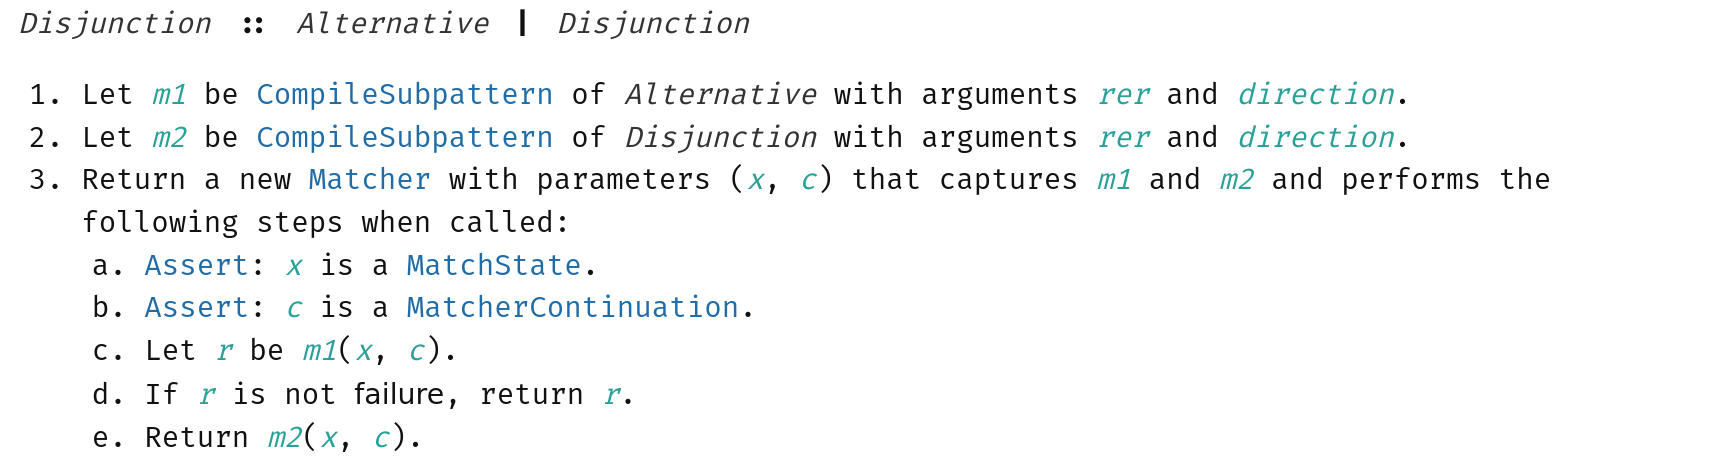
\includegraphics[width=\textwidth]{pics/ecma_spec/disjunction.png}}
                \only<3>{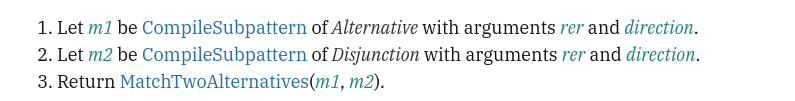
\includegraphics[width=\textwidth]{pics/ecma_spec/disjunction_2024.png}}
            \item<4-> Introduces some additional support for unicode (\texttt{v} flag).
        \end{itemize}        
    \end{frame}

    \begin{frame}{Short-term future work}
        In the near future, we would like to take a look at:
        \pause{}
        \begin{itemize}
            \item Unicode support;
            \pause{}
            \item Integrating with test262;
            \pause{}
            \item
                Additional proofs about the semantics:
                \begin{align*}
                    e\lquestion{} \not\equiv{}& \eps{} \disj{} e \\
                    \pgroup{e\star{}}\star{} \equiv{}& e\star{}\\
                    e\star{} \equiv{}& \eps{} \textup{ where } e \textup{ only ever matches the empty string.}
                \end{align*}
        \end{itemize}
    \end{frame}

    \begin{frame}{Long-term future work}
        \begin{itemize}
            \item Improve the extraction to get a more efficient engine.
            \item Develop a tool to check our comments against the specification.
            \item Prove correct an efficient engine for ECMAScript regexes.
            \item Prove equivalent some alternative semantics more suited for formal reasoning.
        \end{itemize}
    \end{frame}

    \begin{frame}[standout]
        
    \end{frame}
    \appendix

    \section{References}
    \begin{frame}[allowframebreaks]
        \printbibliography[heading=none]{}
    \end{frame}


    \section{Appendix}

    \subsection{Problem 4: mutability}
    \begin{frame}{Getting rid of mutability}
        \begin{center}
            \only<1>{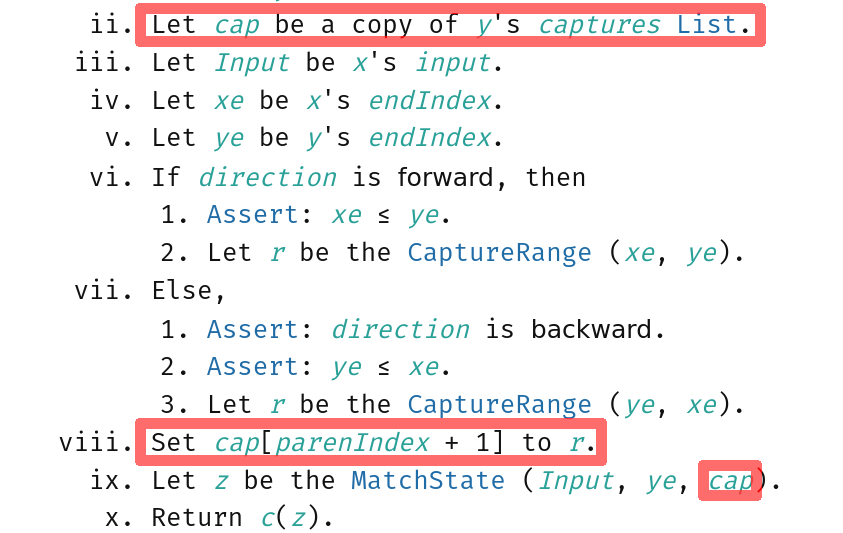
\includegraphics[width=0.8\textwidth]{pics/ecma_spec/set_list/group_hg.png}}
            \only<2>{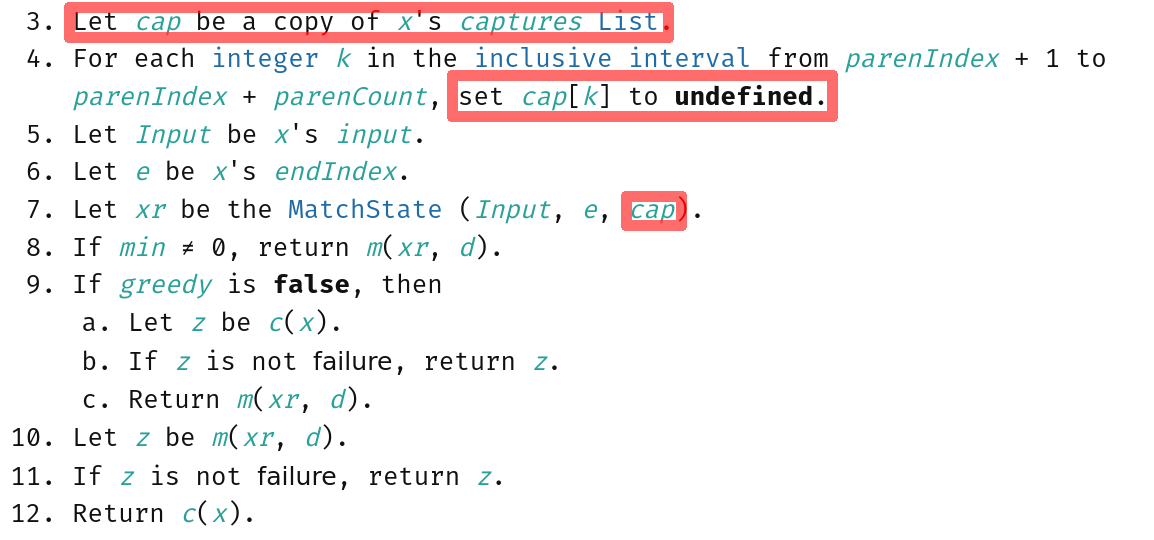
\includegraphics[width=\textwidth]{pics/ecma_spec/set_list/repeat_matcher_hg.png}}
        \end{center}
    \end{frame}

    \subsection{Statistics}
    \begin{frame}{Statistics about the mechanization}
        \centering
        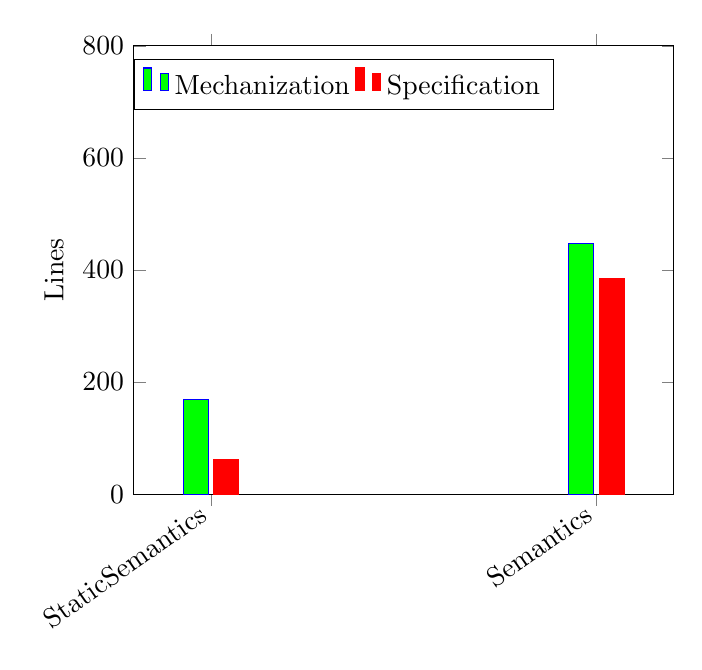
\begin{tikzpicture}
            \begin{axis}[
                ymax=800,
                ymin=0,
                ybar,
                xtick=data,
                legend style={at={(0.39,0.97)},
                   anchor=north,legend columns=2},
                x tick label style={rotate=35,anchor=east},
                symbolic x coords={StaticSemantics, Semantics}, 
                bar width=9pt, 
                enlarge x limits=0.2,
                ylabel={Lines}
                ]
                        \addplot+[ybar, fill=green] plot coordinates {
                            (StaticSemantics, 169)
                            (Semantics, 447)
                        }; 
                        \addplot+[ybar, fill=red] plot coordinates {
                            (StaticSemantics, 62)
                            (Semantics, 385)
                        };
             \legend{\strut Mechanization, \strut Specification}
            \end{axis}
        \end{tikzpicture}
    \end{frame}

    \begin{frame}{Statistics about the proofs}
        \centering
        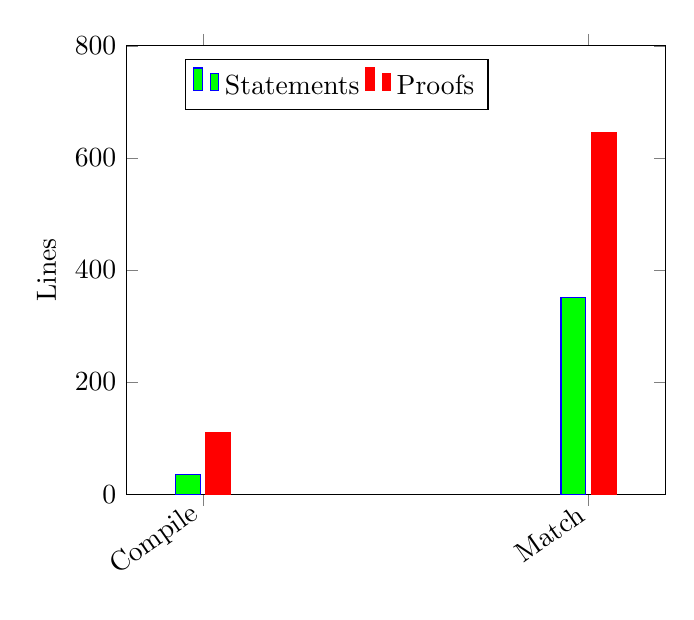
\begin{tikzpicture}
            \begin{axis}[
                ymax=800,
                ymin=0,
                ybar,
                xtick=data,
                legend style={at={(0.39,0.97)},
                   anchor=north,legend columns=2},
                x tick label style={rotate=35,anchor=east},
                symbolic x coords={Compile, Match}, 
                bar width=9pt, 
                enlarge x limits=0.2,
                ylabel={Lines}
                ]
                        \addplot+[ybar, fill=green] plot coordinates {
                            (Compile, 35)
                            (Match, 351)
                        }; 
                        \addplot+[ybar, fill=red] plot coordinates {
                            (Compile, 109)
                            (Match, 645)
                        };
             \legend{\strut Statements, \strut Proofs}
            \end{axis}
        \end{tikzpicture}
    \end{frame}

    \begin{frame}{Raw statistics}
        \lstinputlisting[basicstyle=\scriptsize,xleftmargin=0.1\linewidth,=0.8\linewidth]{listings/stats.txt}
    \end{frame}

\end{document}